\chapter{Diseño hardware}
\label{chap:hard}
\graphicspath{{hard/figs/}{hard/figs/}}

%******************************************************************************************************************************************************


\section{Herramientas de diseño}

Para la implementación hardware del sistema se ha utilizado la herramienta \textit{Altium Desinger}: Altium es un potente entorno de desarrollo que incluye todas las herramientas necesarias durante el proceso de diseño, prueba y fabricación de un prototipo hardware.

\begin{figure}[hbt!]
	\centering
	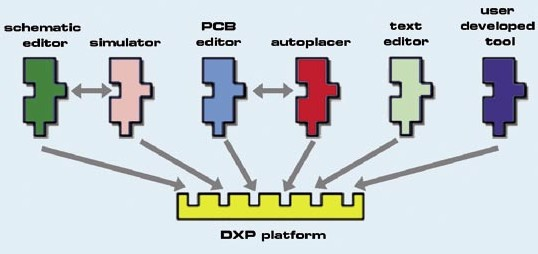
\includegraphics[width=0.7\linewidth]{altium.jpg}
	\caption{Componentes de Altium DPX \citep{Altium}}
	\label{fig::altium}
\end{figure}

Altium es uno de los softwares de diseño hardware más utilizado actualmente por la industria, además cuenta con una gran cantidad de documentación, la cual facilita en uso y el aprendizaje. Todas estas ventajas han hecho que Altium sea la herramienta elegida para desarrollar este apartado del TFG.

Con Altium se han llevado a cabo las tareas de diseño de esquematicos, creación de componentes y footprints, diseño y rutado de la tarjeta y la generación de los ficheros de fabricación. Aunque Altium es un software propietario con un coste elevado, para la realización de los prototipos se han utilizado licencias de prueba del software. 



\section{Elección del hardware}
	\subsection{Integrado CMWX1ZZABZ}
	
	El integrado CMWX1ZZABZ es un módulo diseñado por \textit{Murata}, que incorpora un microcontrolador STM32L0 y un tranceptor de radio SX1276 en el mismo chip. La forma en la que se encuentran conectados ambos módulo en el chip, se resume en la figura  \ref{fig:CMWX1ZZABZ} .
	
	
	\begin{figure}[hbt!]
		\centering
		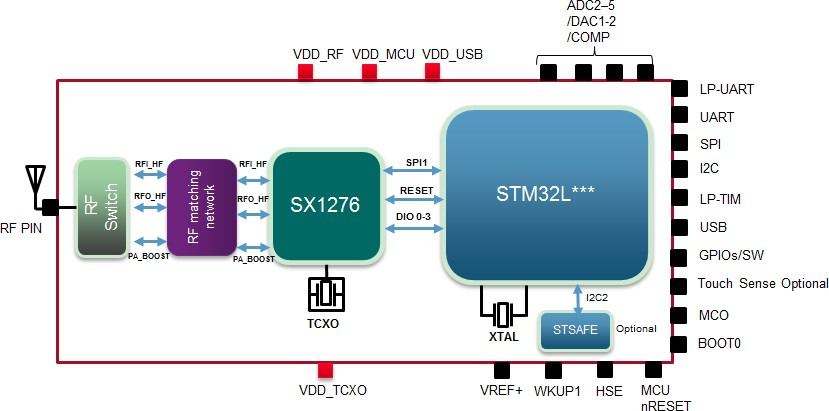
\includegraphics[width = \linewidth]{MurataMCU.jpg}
		\caption{Esquema de bloques del chip CMWX1ZZABZ \citep{Murata}}
		\label{fig:CMWX1ZZABZ}
	\end{figure}
	
	La principal ventaja de este chip, es que reduce en gran medida en espacio utilizado, reduciendo el tamaño final de la tarjeta  y simplificando las conexiones.
	\subsubsection{Microcontrolador STM32L072}
	
	El STM32l072, es un microcontrolador de ultrabajo consumo, diseñado por la empresa \textit{STMicrocontrollers}. Cuenta con una arquitectura de Arm Cortex-M0+ de 32 bits funcionando a 32 MHz, además 192 KB de memoria flash, 6 KB de memoria de datos y 20 KB de memoria RAM \citep{STMpow}. Este microcontralador tiene un amplio abanico de perifericos como SPI, $I^2C$, USART, USB, ADC, USB entre otros. 
	\paragraph{}	
	Lo más destacable de este microcontrolador es ultra-bajo consumo, y sus diferentes modos de funcionamiento, los cuales podemos ver resumido en la figura \ref{fig::powerMCU}. El bajo consumo y altas prestaciones de este chip, lo hacen ideal para este proyecto.
	
	\begin{figure}[hbt!]
		\centering
		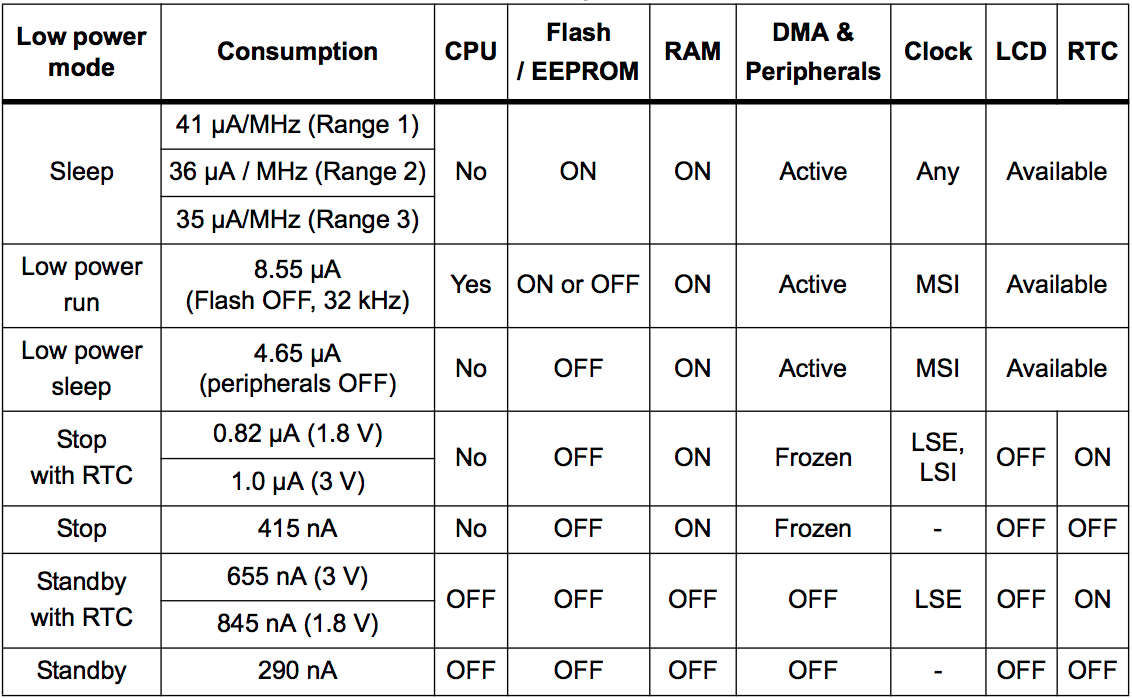
\includegraphics[width = 0.7\linewidth]{powerMCU.png}
		\caption{Consumo y modos de funcionamiento del microcontrolador STM32L072 \citep{STMpow}}
		\label{fig::powerMCU}
	\end{figure}
	
	\subsubsection{Transceptor SX1276}
	
	El SX1276 es un tranceptor de radio, diseñado por \textit{Semtech}, preparado para trabajar con la modulación lora en sistemas de largo alcance y bajo consumo. También puede funcionar como modulador FSK/OOK.
	
	\begin{figure}[hbt!]
		\centering
		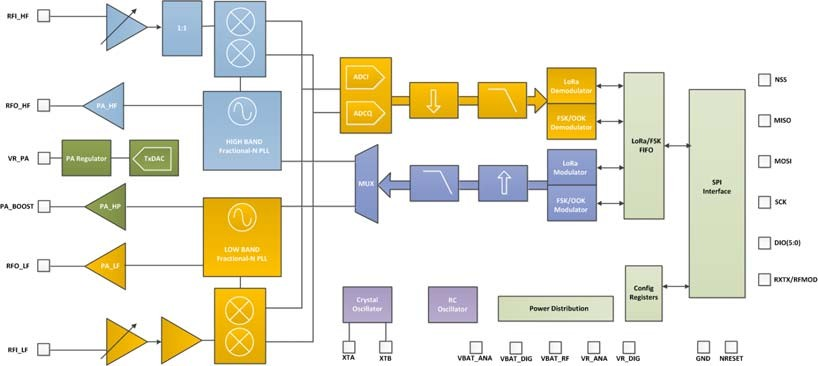
\includegraphics[width = 0.7\linewidth]{sx1276.jpg}
		\caption{Esquema de bloques de la familia de tranceptores SX127x \citep{SX1276}}
	\end{figure}
	
	
	Se carateriza por trabajar en un rango de frecuencias desde 137 MHz hasta los 1020 MHz, con un \textit{"spreading factor"} o factor de enchanchado entre 6 y 12, un ancho de banda entr 7.5 KHz y 500 KHz y una sensibilidad entre -111 dBm y -148 dBm. Con todo esto, consigue velocidades binarias efectivas ente los 18 bps y los 37.5 Kbps \citep{SX1276}.
	\paragraph{}
	Por otro lado, el trasmisor tiene un consumo típico de 10.8 mA en recepción, de entre 20 mA  y 120 mA en recepción (dependiento de la configuración) y un consumo típoco en modo \textit{sleep} de 0.2 uA \citep{SX1276}.
	
	
	\subsection{Conversor analógico/digital AD7194} \label{AD7194}
	
	El AD7194 es un conversor analógico/digital de bajo ruido diseñado para aplicaciones de alta presición. Creado por \textit{Analog}, posee 16 canales de entrada analógicos, una resolución de 24 bits, un reloj interno de 4.92 MHz y un amplificador de entrada de ganacia programable. La comuicación se hace a través de la interfaz SPI del ADC y el SPI-2 del microcontrolador.
	
	\begin{figure}[htb!]
		\centering
		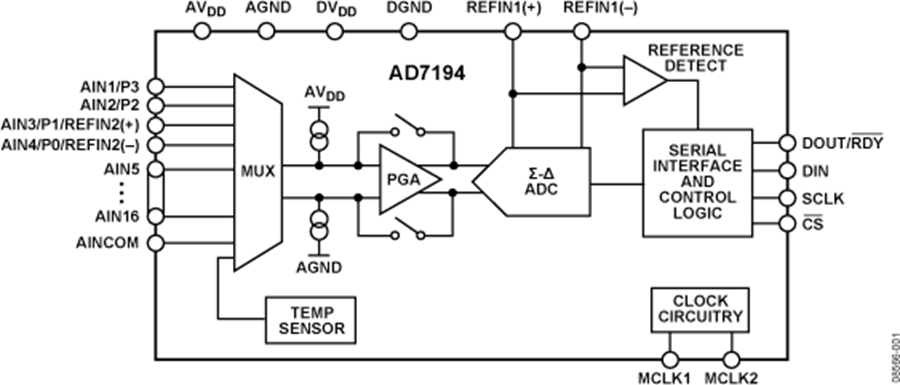
\includegraphics[width=0.7\linewidth]{AD7194.png}
		\caption{Diagrama funcional del AD7194 \citep{AD7194}}
	\end{figure}
	
	Entre sus opciones de configuración, permite la utilización de filtros digitales programables, rechazo de las bandas de 50 Hz y 60 Hz y la utilización de sus canales en modo diferencial (en cualquier configuración) o en modo pseudo-diferencial (tomando como canal negativo GND). Otra de las característica decisivas, es su consumo,  que varia entre los 0.85 mA y los 5.3 mA en función de la ganancia de entrada elegida \citep{AD7194}.
	
	\paragraph{}
	La motivación de usar este ADC, es su aplicación: La medida de termopares. En esta aplicación, se hace necesario una gran presición (las variaciones de tensión en los termopares es muy pequeña) y el bajo ruido de cuantificación. Además, al tener 16 de canales, se pueden utilizar un mayor número de termopares.
	
	
	\subsection{Sensor de temperatura MCP9808T} \label{hard:MCP9808T}
	
	El MCP9808T es un sensor de temperatura digital, que permite medir termperaturas entre -20 ºC y 100 ºC con una presición de  $\pm 0.25 ºC$. Entre su características destaca su comunicación a través de $I^2C$, sus diferentes modos de operación y su bajo consumo, el cual ronda los 200 uA en funcionamiento \citep{MCP9808}.
	
	Su finalidad en el proyecto, será aproximar la temperatura de unión de los conectores a los termopares, la cual es necesaria para realizar una correcta medida (la union de cobre + estaño de los conectores genera una diferencia de potencial parácita que influye en las medidas). A este fenómeno se le llama 
	
	\subsection{Componentes activos} \label{CActive}
	
	Además de los ya mencionados, tambien se ha hecho uso  de otros componentes activos, de los que podemos destacar:
	
	\begin{itemize}
		\item \textbf{Regulador TLV755P: }Es un regulador LDO (\textit{Low-drowput regulator} de sus siglas en inglés) de tension fija a 3.3 V, capaz de dar s su salida hasta 500 mA. Al ser un LDO solo necesita una diferencia de potencial de 238 mV entre sus terminales de entrada y salida, lo que nos permite alimentarlo con una batería de 3.7 V. Otro detalla importante es que su corriente de fugas en reposo es de solo 25 uA, lo que es ideal para mantener el bajo consumo.
		
		\item \textbf{Regulador AD1582BRTZ: }Este regulador es capaz de dar una tensión fija de 2.5 V con una presición muy alta y con una corriente de fugas muy baja. En el proyecto se usará como nivel de referencia del ADC.
		
		\item \textbf{Operacional MCP6001T: }Se trata de un amplificador operaciona de uso general. Funciona con una tensión de alimentación entre 1.8 V y 6 V y tiene un consumo típico de 100 uA. Se utilizará para dar alta impedacia de entrada al circuito de medida de la batería.
		
	\end{itemize}
	
	\subsection{Componentes pasivos}
	
	En este apartado englobamos las resistencias, condensadores e inductancias. De manera general, se ha procurado elegir componentes con un encapsulado SMD de tamaño 0603, el cual es lo suficiente grande para poder soldarlo manualmente sin mucha dificultad.
	
	En cuanto a la resistencias, se han elegido de película de carbono, con una tolerancia del $1 \% $. Por otro lado, los condensadores son, en su mayoría, cerámicos con un dieléctrico X5R ó X7R y una toleracia $\leq 5 \%$. 
	
	\subsubsection{Termopares}
	
	Un termopar es un transductor de temperatura formado por la unión de dos metales diferentes. La variación de temperatura en el punto de unión de los dos metales proboca una varición proporcional de la tensión en el punto de contacto, lo que a su vez genera una corriente eléctrica a través de los condutores. A este efecto termoeléctrico se le conoce como efecto Seedbeck. 
	
	La relación entre la tensión y la temperatura en el termopar se mide mediante el coeficiente de Seedbeck, el cual suele tener unidades de $\mu V / K$. Este coeficiente dependerá de los metales utilizados en la unión, de los cuales dependerán tambien los rangos de temperatura que será capaz de medir el termopar. Las diferentes tipos uniones se distinguen mediante letras como K (NiCr-Ni), E (NiCr-CuNi) o  J (Fe-CuNi). En la gráfica \ref{fig:termCurve} podemos observar las variciones de tensión frente a temperatura de los diferentes tipos de termopares.
	
	\begin{figure}[htb!]
		\centering
		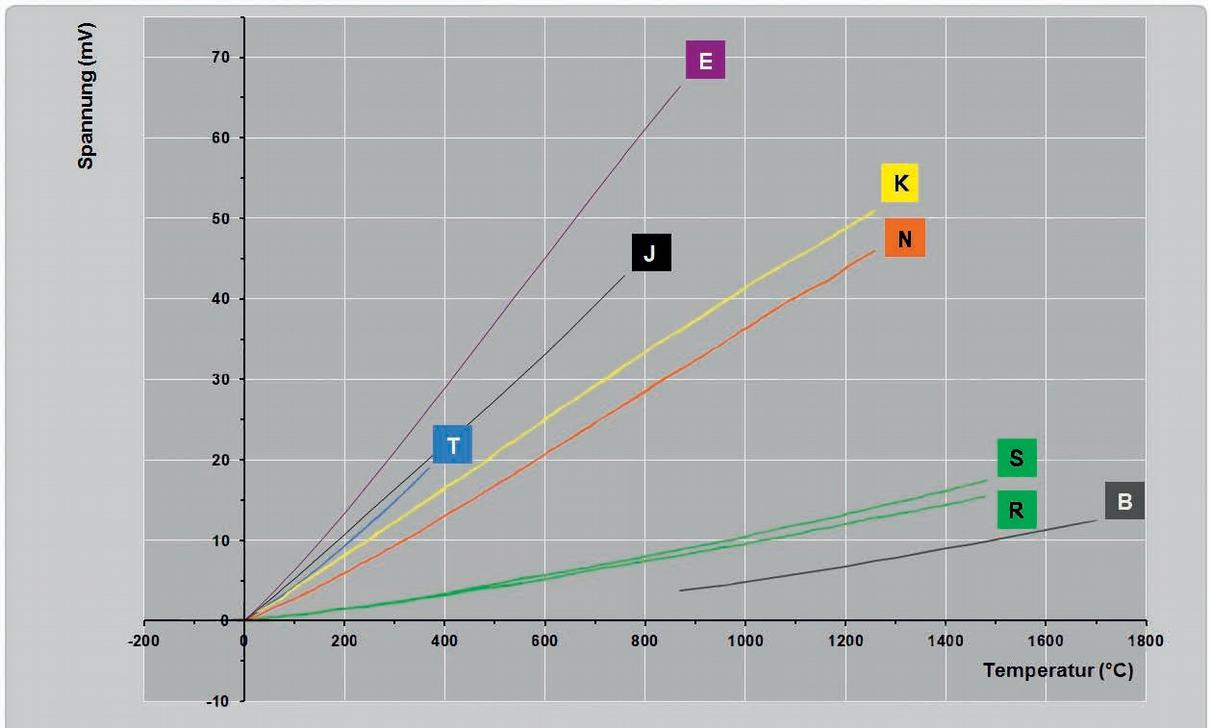
\includegraphics[width = 0.7\linewidth]{termCurve.jpg}
		\caption{Curvas de tensión termoeléctrica}
		\label{fig:termCurve}
	\end{figure}
	
	
	Dado que las medidas se realizan en temperatura ambiente y que la unión cobre-estaño de los conectores forman también un termopar, la medida realizada no se corresponderá con el valor extacto de temperatura. Por ello, para obtener la temperatura absoluta, es necesario realizar una  compensación conocida como "compensacion de la zona fría".
	
\section{Diseño las tarjetas}

	\subsection{Diseño del nodo básico} 
	
		En esta parte se describirá el proceso de diseño un nodo general (sin aplicación específica definida) que contendrá lo necesario para un correcto funcionamiento del microcontrolador y la radio. Uno de los objetivos principales será conseguir un módulo de tamaño reducido que pueda ser facilmente montado en otro circuito impreso. Por esto, se procurará reducir el tamaño de los conectores y pistas y se intentará reducir al máximo el número de componetes.
		
		Para poder utilizar los módulos en placas de expación, se ha optado por un montaje \textit{placa a placa} mediante conectores de borde con \textit{castellated holes} (Agujeros almenados por su traducción al español). Los \textit{castellated holes} son vias (agujeros metalizados que conectan dos capas de un circuito) colocadas en los borde de un circuito impreso las cuales son cortadas para crear medios agujeros metalizados. Estos medios agujeros generalmente son utilizados para conectar de manera sencilla pequeños módulos como si fuesen un componente mas. La fabricación de este tipo de conectores conlleva un proceso especial, lo que eleva el precio de fabricación de los prototipos.

	\begin{figure}[htb!]
		\centering
		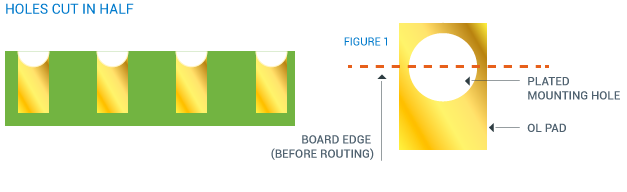
\includegraphics[width= 0.6\linewidth]{castellated-holes.png}
		\caption{Castellated holes}
		\label{fig:castellated}
	\end{figure}
El módulo tambien cuenta con algunos elemetos de depuración, como los diodos LED D1 y D2 (sección \ref{hard:nodeSCH}), conectados a 3.3V y al GPIO PA0 del microcontrolador respectivamente. También cuenta con botón el cual, al ser pulsado, conecta el pin NRESET a tierra reiniciando el microcontrolador (el pin es activo a nivel bajo según la especificación del fabricante \ref{fig:CMWX1ZZABZ}).

Para su programación y depuración, se han añadido 5 pads, con una separación de 1.27 mm, conectados a la alimentación y a la interfaz SWD (\textit{Serial Wire Debug} por sus siglas en ingés) del microcontrolador. Mediante estos pads y un el programador STLINK, podemos crear una conexión con la herramienta de depuracón GDB, la cual veremos en la sección \ref{soft:debugApp} de este documento.

La antena va conectada al nodo mediante un conector miniatura del tipo U.LF. Los conectores U.LF, trabajan en un amplio rango de frecuencias (hasta los 6 GHz), por lo que es habitual verlos en tarjetas miniPCI WiFi o en módulos GPS. Ante la imposibilidad de conseguir una buena adaptación de impedancias entre el microcontrolador y la antena (lo que causará perdidas de retorno en la línea de transmición), se ha procurado reducir la longitud de la pista que los une y se han añadido los pads para conectar una red de adaptación en el caso de que fuese necesario (componentes L1, L2 y C6 de esquemático de la sección \ref{hard:nodeSCH}).
				
		
		\pagebreak

		\subsubsection{Esquemáticos} \label{hard:nodeSCH}
	\begin{figure}[hbt!]
		\centering
		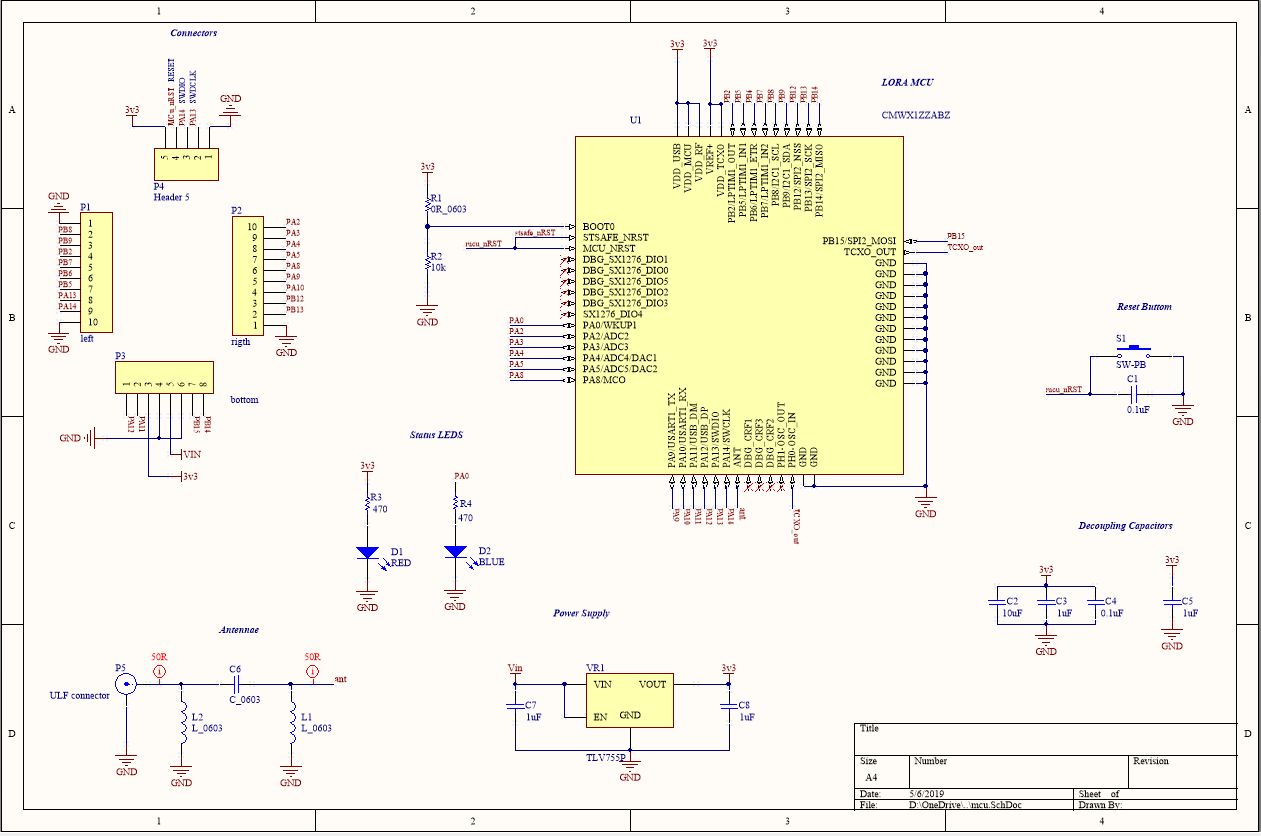
\includegraphics[angle= 90, width = \linewidth]{lora_1.PNG}
		\caption{Esquemáticos de la tarjeta de expanción.}
		\label{fig:car13}
	\end{figure}		
	\pagebreak


		\subsubsection{Layout} \label{hard:nodeLay}
		
		
		\begin{figure}[htb!]
            \centering
            \hfill
            \begin{subfigure}[t]{0.35\textwidth}
                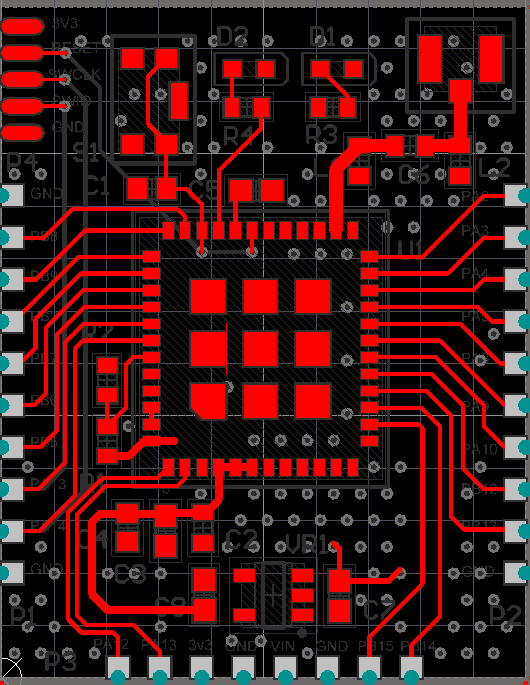
\includegraphics[width = \linewidth]{lora_6.PNG}
                \caption{Elementos de la capa superior.}
            \end{subfigure}%
            \hfill
            \begin{subfigure}[t]{0.35\textwidth}
                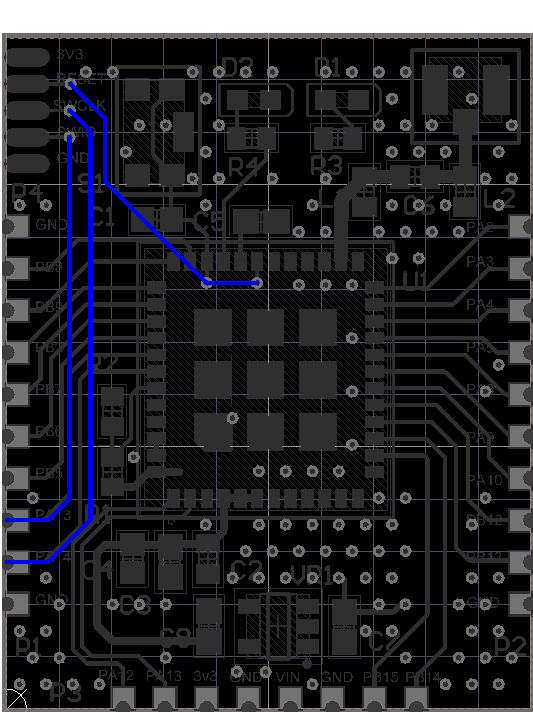
\includegraphics[width = \linewidth]{lora_7.PNG}
                \caption{Elementos de la capa inferior.}
            \end{subfigure}
            \hfill
            \begin{subfigure}[t]{0.35\textwidth}
    			\centering
    			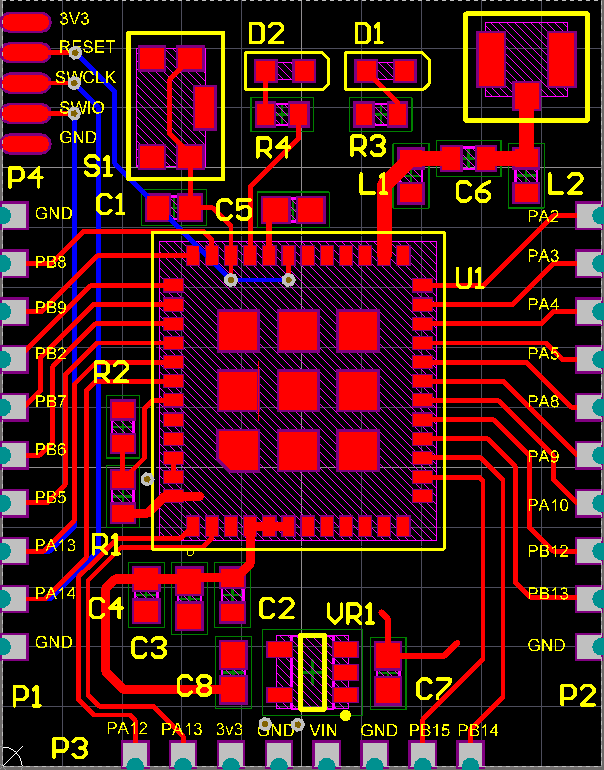
\includegraphics[width =\linewidth]{lora_5.PNG}
    			\caption{PCB con todas las capas}
    		\end{subfigure}
    		
    		\caption{Estructura de la PCB}
    		\label{fig:PCBnode}

        \end{figure}
        
        
        El resultado obtenido es una tarjeta de 32x25 mm de lóngitud como la monstrada en la figura \ref{fig:PCBnode}, la cual se ha diseñado con solo dos capas para reducir los costes y tiempo de fabricación.Como se puede apreciar, todos lo componentes se encuentran situados en la capa superior de la PCB, esto se ha hecho con el fin de poder usar la PCB como un módulo de montaje superficial. 
        
        Para reducir los efectos de capacitancias parásitas y autoinductancias entre las pistas, ambas capas cuentan con un plano de masa que cubre todas las zonas libres del circuito. Ambos planos están conectados mediante un gran número de vias (también llamado \textit{via stitching}), la cuales ofrecen una línea de retorno rápido para las corrientes, evitan bucles en la masa y evitan que los planos funcionen como antenas. Estos planos se han ocultado en la figura \ref{fig:PCBnode} para facilitar la visualización de las pistas y componentes.
        
	\subsection{Diseño de la tarjeta de expación}
	
	Con el nodo básico funcionando, el objetivo ahora es darle una aplicación específica. Para ello, se diseñará una tarjeta de expanción con sensores con las siguientes características:
	
	\begin{itemize}
		\item 6 entradas para termopares 
		\item 3 entradas analógicas
		\item Sensor de temperatura cerca de los conectores
		\item Conectores enchufables con clemas
		\item Sensor de batería
		\item ADC de alta presición 
		\item Posibilidad de cortar la alimentación
		
	\end{itemize}	
	
	Como ADC se ha utilizado un AD7194 como el descrito el descrito en la sección \ref{AD7194}, el cual cuenta con el suficiente número de canales para soportar los 6 termopares, las 3 entradas analógicas y el sensor de la batería. Para medir la temperatura de unión se ha utilizado un sensor de temperatura MCP9808T, descrito en la seicción \ref{hard:MCP9808T}. En los siguientes apartados se describiran de forma más detallada los esquemas utilizados para la medida de los termopares, entradas analógicas, batería y alimentación de la placa.
	
		\subsubsection{Medida de los termopares}	
	
		Para acondicionar la entrada se ha utilizado la estructura mostrada en la figura \ref{fig:car10}.
	
	\begin{figure}[hbt!]
		\centering
		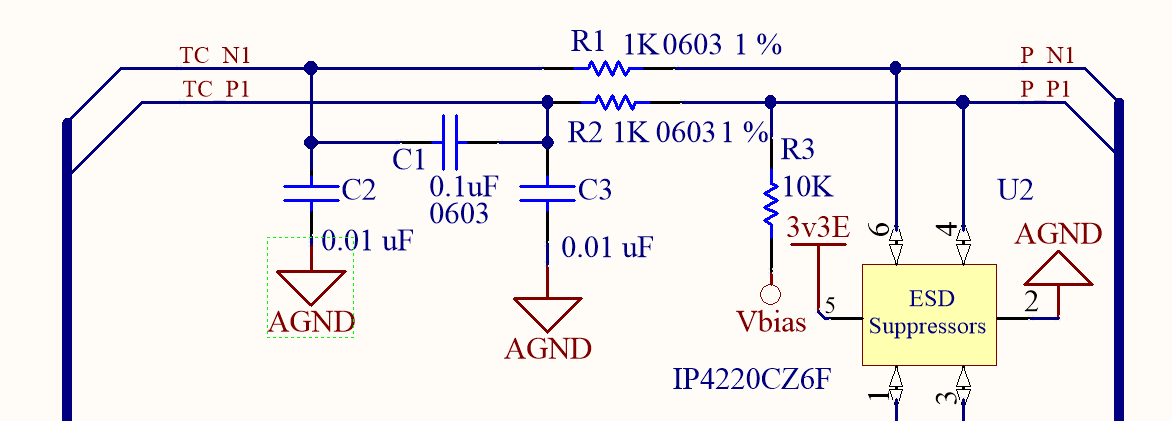
\includegraphics[width = \linewidth ]{carrier_10.PNG}
		\caption{Circuito acondicionador de entrada de los termopares.}
		\label{fig:car10}
	\end{figure}
		
	Los pares R1-C2 y R2-C3, forman dos filtros paso bajo, que filtrarán las entradas en como común del termopar, eliminando el ruido presente en el termopar y evitando el alisasing en el ADC. Sabiendo que R1 = R2 = R y que C1 = C2 = C, obtenemos que la frecuencia de corte del filtro viene dada por la expresión:
	
	\begin{equation}
		f_c = \frac{1}{2\times \pi\times R\times C} \approx 16 KHz
	\end{equation}
	
	Al no ser ideales, los componentes son iguales, lo que genera una perturbación en el modo diferencial de la señal, lo que a su vez desemboca en una dísminución del ratio de rechazo al modo común o CMRR (\textit{Common Mode Reject Ratio} por sus siglas en inglés). Como la medida de termopares requiere un alto CMRR, se ha añadido un filtro diferencial, formado por C1, R1 y R2, que compenza los efectos de los filtros en modo común. La frecuencia de corte de este filtro viene dado por la ecuación:
		\begin{equation}
		f_c = \frac{1}{2\times \pi\times (R_1 + R_2)\times C_1} \approx 16 KHz
	\end{equation}
	
	
		\subsubsection{Medida de entradas analógicas}

Para las entradas analógicas, se ha utilizado el circuito acondicionador de la entrada de la figura \ref{fig:car11}.

\begin{figure}[hbt!]
	\centering
	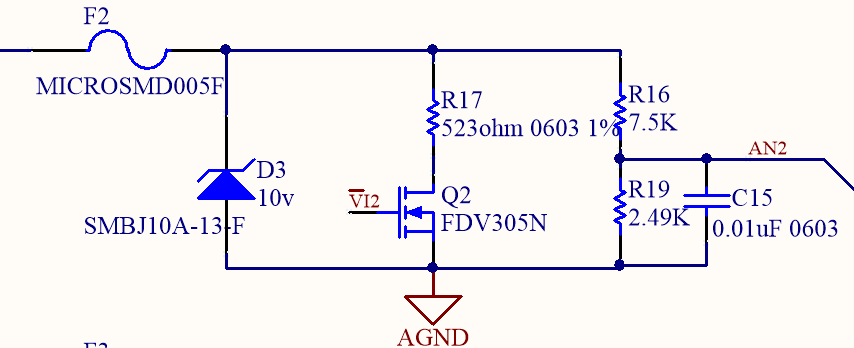
\includegraphics[width = \linewidth]{carrier_11.PNG}
	\caption{Circuito acondicionador de las entradas analógicas.}
	\label{fig:car11}
\end{figure}

\paragraph{}
las resistencias R16 y R19, conforman un divisor resistivo con una atenuación de 1/4 de la tensión de entrada. Teniendo en cuenta que utilizamos un regulador AD1582BRTZ a 2.5 V (como el especificado en la sección \ref{CActive}), conseguimos un margen dinámico a la entrada de 10 V.
\paragraph{}
Por otro lado, con la conmutación del transistor Q2, consegimos que la impedacia de entrada sea aproximadamente de $ 523 \omega $, lo que permite la medida de entradas en corriente de hasta 20 mA. La expresión de la  corriente a la entrada se puede expresar de la forma:

\pagebreak

\begin{equation}
	i_e \approx \frac{4V_m - V_{DS} }{R_{17}}
\end{equation}

siendo:
\begin{itemize}
	\item $V_m$ tensión medida en el ADC
	\item $V_{DS}$ tensión \textit{Drain-Source} del transistor
\end{itemize}


El circuito tambien cuenta con protección a su entrada: El fusible F2 limita la corriente de entrada del circuito a un máximo de 50 mA. A su vez, el diodo zener D3 limita la tensión máxima a la entrada de 10 v. En el caso de que la entrada superase los 50 mA, el fusible mantendría una corriente contante de 50 mA hasta superar el tiempo de ruptura $T_r$ (aproximadamente 100 ms según las especificaciones del fabricante).
		
		\subsubsection{Media del nivel de batería}

Para medir el nivel de tensión de la batería, se ha utilizado en circuito de la figura \ref{fig:car12}.

\begin{figure}[hbt!]
	\centering
	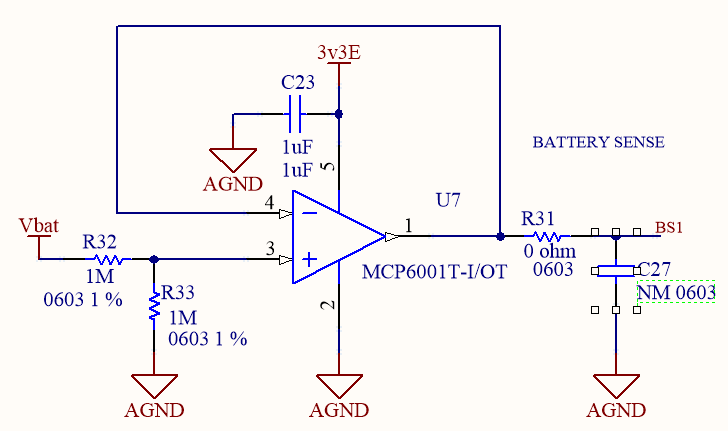
\includegraphics[width = 0.7\linewidth]{carrier_12.PNG}
	\caption{Circuito de medida de la batería.}
	\label{fig:car12}
\end{figure}			
		
Las resistencias R32 y R33 del circuito forma un divisor resistivo con una atenuación de 1/2. El amplificador operacional, el cual se encuentra con una configuración de seguidor de tensión, proporciona una entrada en alta impedancia (evitando así derivas de corriente). Como las resistencias estan el rango de los mega ohmios, la corriente que circula desde la batería tomará valores de micro amperios, disminuyendo el consumo de batería.

Por último, la resistencia R31 y condensador C27 dan la posibilidad de poner un filtro paso bajo si fuese necesario. Este filtro funcionaría como filtro anti-alisaing, evitando errores en las medidas del ADC.

		\subsubsection{Alimentación de los componentes}
		
Para alimentar la tarjeta, se ha utilizado un regulador TLV755P como el detallado en la sección \ref{CActive}, cuya activación se puede controlar desde microcontrolador mediante el pin de \textit{ENABLE}. Mediante las resistencias R34 y R35 se puede elegir entre tener el regulador siempre activo o controlarlo desde el microcontrolador.  

\begin{figure}[hbt!]
	\centering
	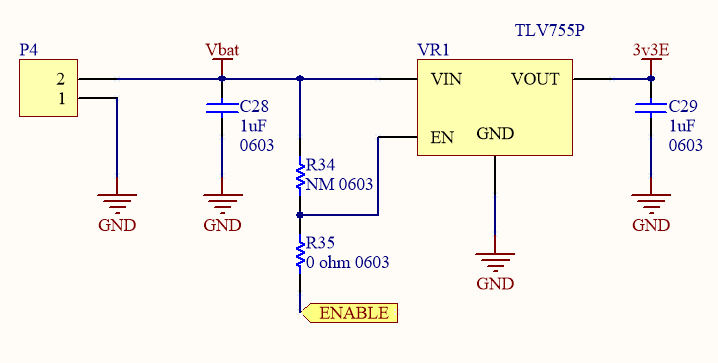
\includegraphics[width = 0.7\linewidth]{carrier_8.PNG}
	\caption{Circuito de alimentación de la tarjeta de expación.}
\end{figure}
		
Con el fin de eliminar el ruido de conmutación presentes en la alimentación y mejorar la presición del ADC, se han separado la alimentación analógica de la digital mediante el filtro de la figura \ref{fig:car9}.

\begin{figure}[hbt!]
	\centering
	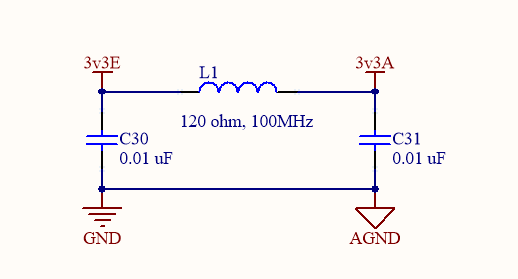
\includegraphics[width = 0.7\linewidth]{carrier_9.PNG}
	\caption{Filtro de la alimentación}
	\label{fig:car9}
\end{figure}
\pagebreak

		\subsubsection{Esquemáticos}
\begin{figure}[hbt!]
	\centering
	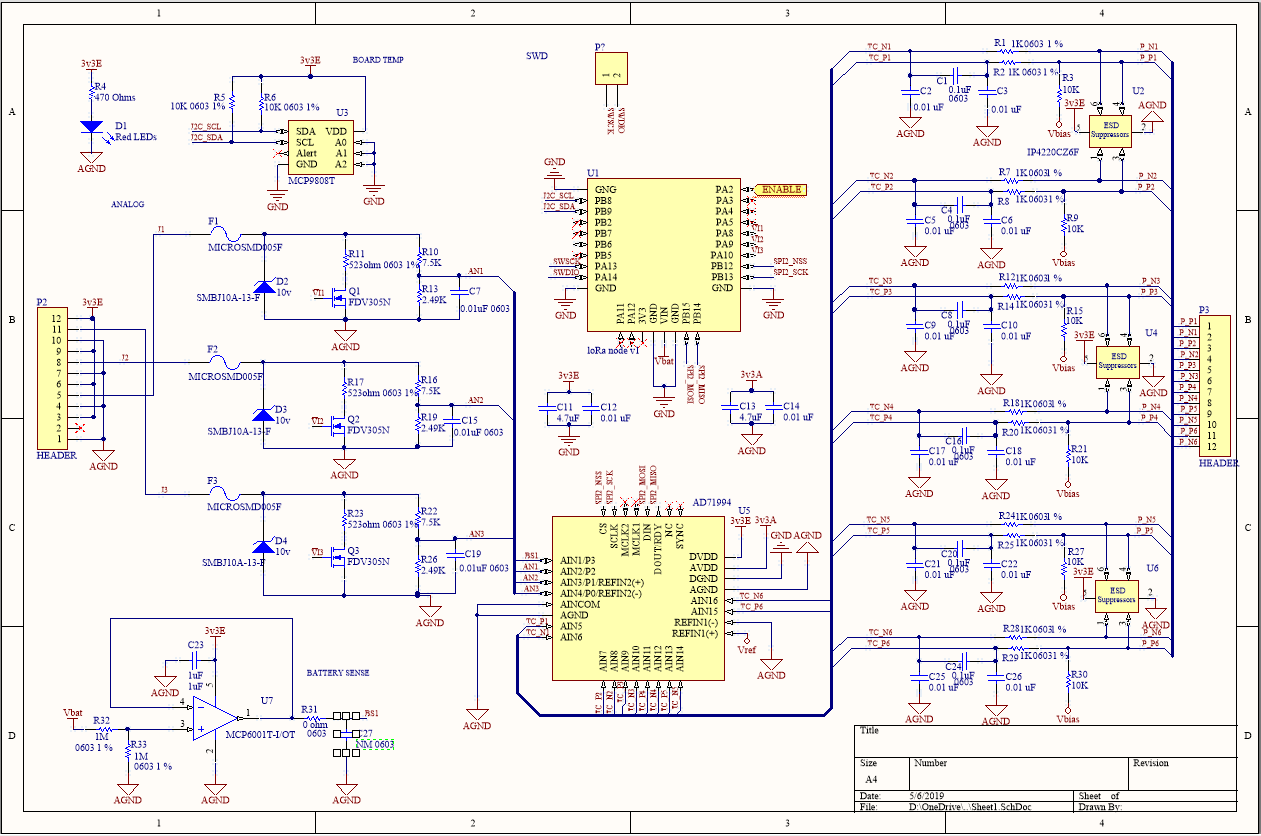
\includegraphics[angle= 90, width = \linewidth]{carrier_13.PNG}
	\caption{Esquemáticos de la tarjeta de expanción.}
	\label{fig:car13}
\end{figure}		
\pagebreak
		\subsubsection{Layout}
		
A la hora de diseñar la PCB, se han colocado los componentes en bloques funcionales, procurando acortar el tamano de las pistas. La disposición de los bloques funcionales en la PCB se  ha hecho intentando reducir al máximo el espacio ocupado e intentando utilizar pistas simples y con conexión directa entre componentes. El sensor de temperatura MCP9808T se ha situado en una zona cercana a los conectores de los termopares para medir con mayor presición la temperatura de unión. 

     	\begin{figure}[htb!]
            \centering
            
            \begin{subfigure}[t]{0.45\textwidth}
                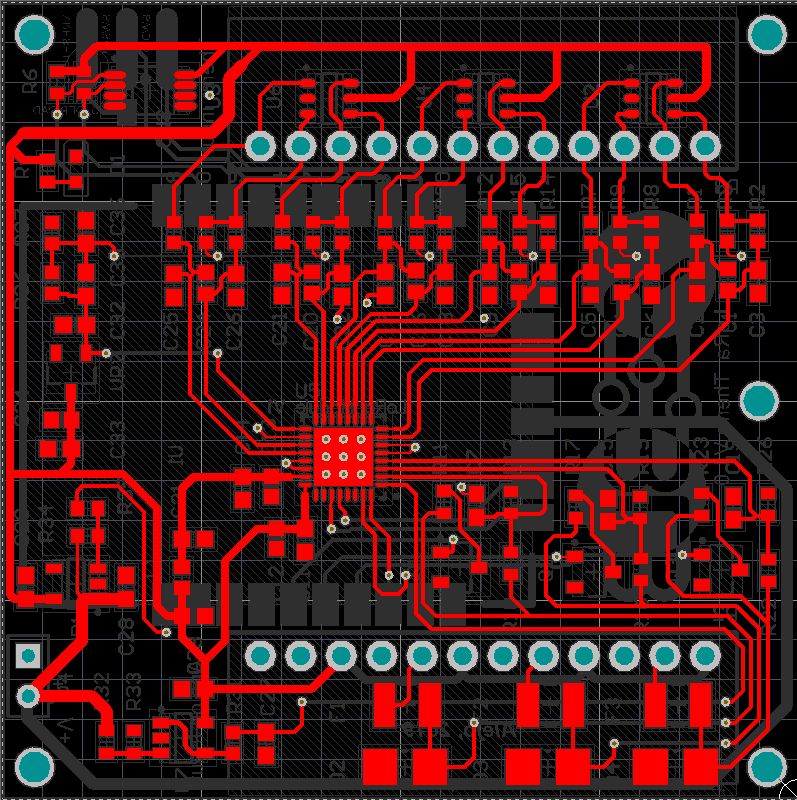
\includegraphics[width = \linewidth]{carrier_2.PNG}
                \caption{Elementos de la capa superior.}
            \end{subfigure}%
            \hfill
            \begin{subfigure}[t]{0.45\textwidth}
                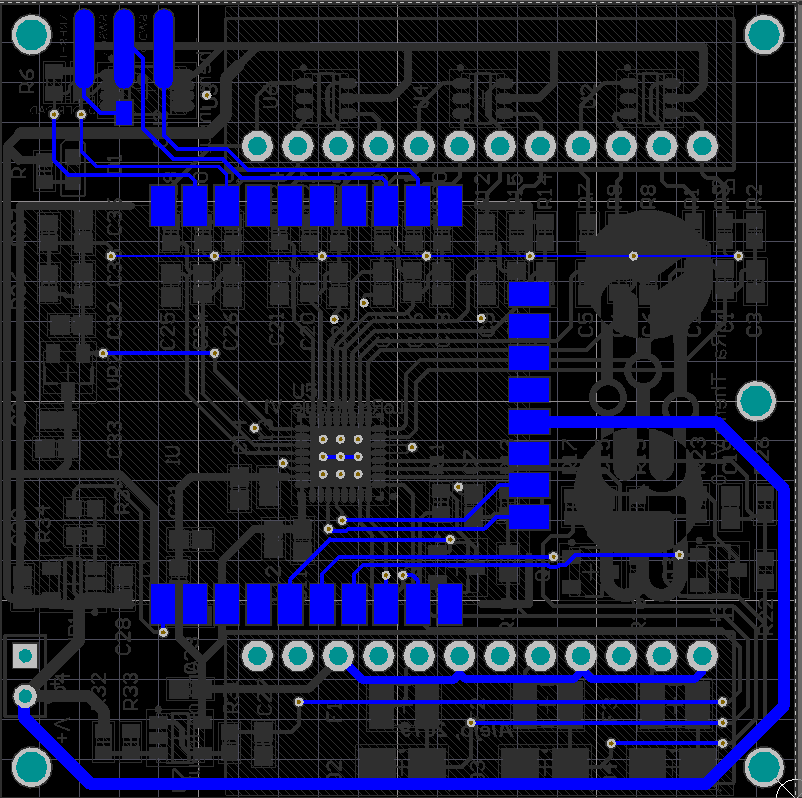
\includegraphics[width = \linewidth]{carrier_3.PNG}
                \caption{Elementos de la capa inferior.}
            \end{subfigure}
            
            \begin{subfigure}[t]{0.5\textwidth}
    			\centering
    			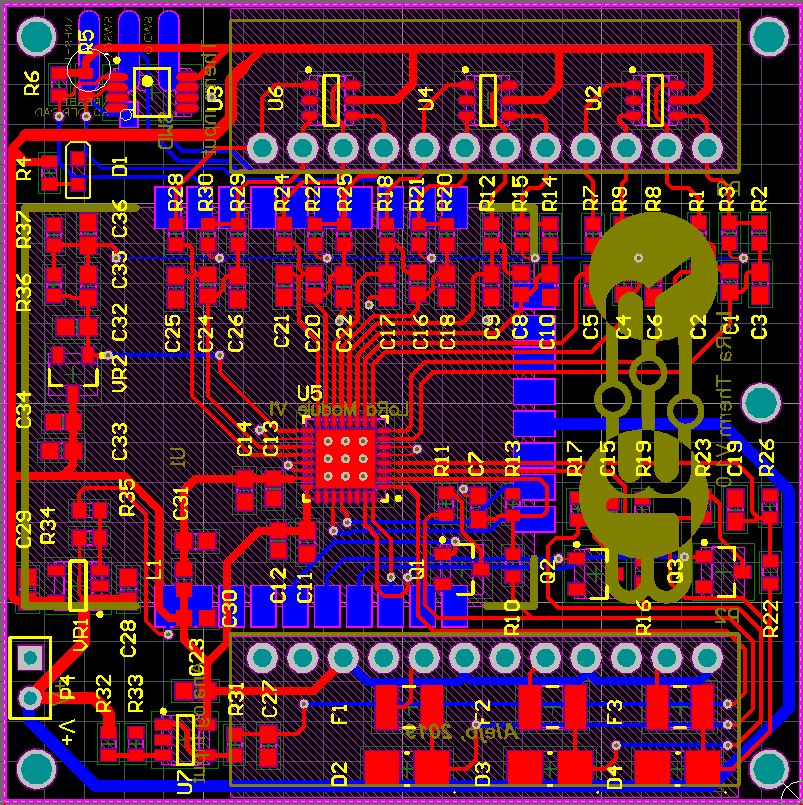
\includegraphics[width =\linewidth]{carrier_1.PNG}
    			\caption{PCB con todas las capas}
    		\end{subfigure}
    		
    		\caption{Estructura de la PCB}
    		\label{fig:PCBcarrier}

        \end{figure}

Al igual que en los nodo vistos en la sección \ref{hard:nodeLay}, esta placa está diseñada a dos capas y cuenta con dos planos de masa, en amabas caras del circuito, con el fin de evitar efectos parásitos en las líneas de transmisión. El resutado, es una PCB de 50x50 mm, cuya disposición de componentes se encuntra en la figura \ref{fig:PCBcarrier}.
		
\section{Lista de componentes}
	
	
\begin{table}[htb!]

\centering

\begin{tabular}{|l|l|l|l|}
\hline
Description            & Designator     & Part Number        & Value  \\ \hline
Capacitor              & C1, C4         & C0603C104J3RAC     & 0.1uF  \\ \hline
Capacitor              & C2             & GRM188R60J106KE47D & 10uF   \\ \hline
Capacitor              & C3, C5, C7, C8 & 885012206052       & 1uF    \\ \hline
INFRARED GaAs LED      & D1             & 150060RS75000      & Red    \\ \hline
INFRARED GaAs LED      & D2             & 150060BS75000      & NM     \\ \hline
BNC Elbow Connector    & P5             & CONUFL001-SMD      &        \\ \hline
Resistor               & R2             & RC0603FR-0710KL    & 10K    \\ \hline
Resistor               & R3, R4         & AC0603FR-13470RL   & 470ohm \\ \hline
Switch                 & S1             & TL6330AF200Q       &        \\ \hline
RF MODULE              & U1             & CMWX1ZZABZ-078     &        \\ \hline
LDO Voltage Regulators & VR1            & TLV75533PDBVR      &        \\ \hline
\end{tabular}
\caption{Componentes del nodo básico}
\label{tab:nodeBOM}

\end{table}

\begin{table}[htb!]

\centering

\begin{tabular}{|l|l|l|l|}
\hline
Description       & Designator                                                                                                                   & Part Number       & Value                                                         \\ \hline
Capacitors        & C1, C4, C8, C16, C20, C24                                                                                                    & C0603C104J3RAC    & 0.1uF                                                         \\ \hline
Capacitors        & \begin{tabular}[c]{@{}l@{}}C2, C3, C5, C6, C9, C10, \\ C12, C14, C17, C18, C21, \\ C22, C25, C26, C30, C31, C33\end{tabular} & 885012206089      & 0.01 uF                                                       \\ \hline
Capacitors        & C7, C15, C19                                                                                                                 & 885012206089      & 0.01uF                                                        \\ \hline
Capacitors        & C11, C13, C34                                                                                                                & JMK107BJ475KA-T   & 4.7uF                                                         \\ \hline
Capacitors        & C23, C28, C29, C32, C35, C36                                                                                                 & 885012206052      & 1uF                                                           \\ \hline
INFRARED GaAs LED & D1                                                                                                                           & 150060RS75000     & 10V                                                           \\ \hline
ESD Suppressors   & D2, D3, D4                                                                                                                   & SMBJ10A-13-F      &                                                               \\ \hline
Resettable Fuses  & F1, F2, F3                                                                                                                   & MICROSMD005F-2    &                                                               \\ \hline
Ferrite Beads     & L1                                                                                                                           & 2506031217Z0      & \begin{tabular}[c]{@{}l@{}}120 ohm, \\ \\ 100MHz\end{tabular} \\ \hline
MOSFET            & Q1, Q2, Q3                                                                                                                   & FDV305N           &                                                               \\ \hline
Resistors         & \begin{tabular}[c]{@{}l@{}}R1, R2, R7, R8, R12, R14, R18,\\ R20, R24, R25, R28, R29, \\ R36, R37\end{tabular}                & CRCW06031K00FKEAC & 1K                                                            \\ \hline
\end{tabular}
\caption{Componentes de la placa de expanción}
\label{tab:termBOM}
\end{table}
	
\section{Fabricación y montaje}



